% Options for packages loaded elsewhere
\PassOptionsToPackage{unicode}{hyperref}
\PassOptionsToPackage{hyphens}{url}
\PassOptionsToPackage{dvipsnames,svgnames,x11names}{xcolor}
%
\documentclass[
  letterpaper,
  DIV=11,
  numbers=noendperiod]{scrartcl}

\usepackage{amsmath,amssymb}
\usepackage{lmodern}
\usepackage{iftex}
\ifPDFTeX
  \usepackage[T1]{fontenc}
  \usepackage[utf8]{inputenc}
  \usepackage{textcomp} % provide euro and other symbols
\else % if luatex or xetex
  \usepackage{unicode-math}
  \defaultfontfeatures{Scale=MatchLowercase}
  \defaultfontfeatures[\rmfamily]{Ligatures=TeX,Scale=1}
\fi
% Use upquote if available, for straight quotes in verbatim environments
\IfFileExists{upquote.sty}{\usepackage{upquote}}{}
\IfFileExists{microtype.sty}{% use microtype if available
  \usepackage[]{microtype}
  \UseMicrotypeSet[protrusion]{basicmath} % disable protrusion for tt fonts
}{}
\makeatletter
\@ifundefined{KOMAClassName}{% if non-KOMA class
  \IfFileExists{parskip.sty}{%
    \usepackage{parskip}
  }{% else
    \setlength{\parindent}{0pt}
    \setlength{\parskip}{6pt plus 2pt minus 1pt}}
}{% if KOMA class
  \KOMAoptions{parskip=half}}
\makeatother
\usepackage{xcolor}
\setlength{\emergencystretch}{3em} % prevent overfull lines
\setcounter{secnumdepth}{-\maxdimen} % remove section numbering
% Make \paragraph and \subparagraph free-standing
\ifx\paragraph\undefined\else
  \let\oldparagraph\paragraph
  \renewcommand{\paragraph}[1]{\oldparagraph{#1}\mbox{}}
\fi
\ifx\subparagraph\undefined\else
  \let\oldsubparagraph\subparagraph
  \renewcommand{\subparagraph}[1]{\oldsubparagraph{#1}\mbox{}}
\fi

\usepackage{color}
\usepackage{fancyvrb}
\newcommand{\VerbBar}{|}
\newcommand{\VERB}{\Verb[commandchars=\\\{\}]}
\DefineVerbatimEnvironment{Highlighting}{Verbatim}{commandchars=\\\{\}}
% Add ',fontsize=\small' for more characters per line
\usepackage{framed}
\definecolor{shadecolor}{RGB}{241,243,245}
\newenvironment{Shaded}{\begin{snugshade}}{\end{snugshade}}
\newcommand{\AlertTok}[1]{\textcolor[rgb]{0.68,0.00,0.00}{#1}}
\newcommand{\AnnotationTok}[1]{\textcolor[rgb]{0.37,0.37,0.37}{#1}}
\newcommand{\AttributeTok}[1]{\textcolor[rgb]{0.40,0.45,0.13}{#1}}
\newcommand{\BaseNTok}[1]{\textcolor[rgb]{0.68,0.00,0.00}{#1}}
\newcommand{\BuiltInTok}[1]{\textcolor[rgb]{0.00,0.23,0.31}{#1}}
\newcommand{\CharTok}[1]{\textcolor[rgb]{0.13,0.47,0.30}{#1}}
\newcommand{\CommentTok}[1]{\textcolor[rgb]{0.37,0.37,0.37}{#1}}
\newcommand{\CommentVarTok}[1]{\textcolor[rgb]{0.37,0.37,0.37}{\textit{#1}}}
\newcommand{\ConstantTok}[1]{\textcolor[rgb]{0.56,0.35,0.01}{#1}}
\newcommand{\ControlFlowTok}[1]{\textcolor[rgb]{0.00,0.23,0.31}{#1}}
\newcommand{\DataTypeTok}[1]{\textcolor[rgb]{0.68,0.00,0.00}{#1}}
\newcommand{\DecValTok}[1]{\textcolor[rgb]{0.68,0.00,0.00}{#1}}
\newcommand{\DocumentationTok}[1]{\textcolor[rgb]{0.37,0.37,0.37}{\textit{#1}}}
\newcommand{\ErrorTok}[1]{\textcolor[rgb]{0.68,0.00,0.00}{#1}}
\newcommand{\ExtensionTok}[1]{\textcolor[rgb]{0.00,0.23,0.31}{#1}}
\newcommand{\FloatTok}[1]{\textcolor[rgb]{0.68,0.00,0.00}{#1}}
\newcommand{\FunctionTok}[1]{\textcolor[rgb]{0.28,0.35,0.67}{#1}}
\newcommand{\ImportTok}[1]{\textcolor[rgb]{0.00,0.46,0.62}{#1}}
\newcommand{\InformationTok}[1]{\textcolor[rgb]{0.37,0.37,0.37}{#1}}
\newcommand{\KeywordTok}[1]{\textcolor[rgb]{0.00,0.23,0.31}{#1}}
\newcommand{\NormalTok}[1]{\textcolor[rgb]{0.00,0.23,0.31}{#1}}
\newcommand{\OperatorTok}[1]{\textcolor[rgb]{0.37,0.37,0.37}{#1}}
\newcommand{\OtherTok}[1]{\textcolor[rgb]{0.00,0.23,0.31}{#1}}
\newcommand{\PreprocessorTok}[1]{\textcolor[rgb]{0.68,0.00,0.00}{#1}}
\newcommand{\RegionMarkerTok}[1]{\textcolor[rgb]{0.00,0.23,0.31}{#1}}
\newcommand{\SpecialCharTok}[1]{\textcolor[rgb]{0.37,0.37,0.37}{#1}}
\newcommand{\SpecialStringTok}[1]{\textcolor[rgb]{0.13,0.47,0.30}{#1}}
\newcommand{\StringTok}[1]{\textcolor[rgb]{0.13,0.47,0.30}{#1}}
\newcommand{\VariableTok}[1]{\textcolor[rgb]{0.07,0.07,0.07}{#1}}
\newcommand{\VerbatimStringTok}[1]{\textcolor[rgb]{0.13,0.47,0.30}{#1}}
\newcommand{\WarningTok}[1]{\textcolor[rgb]{0.37,0.37,0.37}{\textit{#1}}}

\providecommand{\tightlist}{%
  \setlength{\itemsep}{0pt}\setlength{\parskip}{0pt}}\usepackage{longtable,booktabs,array}
\usepackage{calc} % for calculating minipage widths
% Correct order of tables after \paragraph or \subparagraph
\usepackage{etoolbox}
\makeatletter
\patchcmd\longtable{\par}{\if@noskipsec\mbox{}\fi\par}{}{}
\makeatother
% Allow footnotes in longtable head/foot
\IfFileExists{footnotehyper.sty}{\usepackage{footnotehyper}}{\usepackage{footnote}}
\makesavenoteenv{longtable}
\usepackage{graphicx}
\makeatletter
\def\maxwidth{\ifdim\Gin@nat@width>\linewidth\linewidth\else\Gin@nat@width\fi}
\def\maxheight{\ifdim\Gin@nat@height>\textheight\textheight\else\Gin@nat@height\fi}
\makeatother
% Scale images if necessary, so that they will not overflow the page
% margins by default, and it is still possible to overwrite the defaults
% using explicit options in \includegraphics[width, height, ...]{}
\setkeys{Gin}{width=\maxwidth,height=\maxheight,keepaspectratio}
% Set default figure placement to htbp
\makeatletter
\def\fps@figure{htbp}
\makeatother

\KOMAoption{captions}{tableheading}
\makeatletter
\makeatother
\makeatletter
\makeatother
\makeatletter
\@ifpackageloaded{caption}{}{\usepackage{caption}}
\AtBeginDocument{%
\ifdefined\contentsname
  \renewcommand*\contentsname{Table of contents}
\else
  \newcommand\contentsname{Table of contents}
\fi
\ifdefined\listfigurename
  \renewcommand*\listfigurename{List of Figures}
\else
  \newcommand\listfigurename{List of Figures}
\fi
\ifdefined\listtablename
  \renewcommand*\listtablename{List of Tables}
\else
  \newcommand\listtablename{List of Tables}
\fi
\ifdefined\figurename
  \renewcommand*\figurename{Figure}
\else
  \newcommand\figurename{Figure}
\fi
\ifdefined\tablename
  \renewcommand*\tablename{Table}
\else
  \newcommand\tablename{Table}
\fi
}
\@ifpackageloaded{float}{}{\usepackage{float}}
\floatstyle{ruled}
\@ifundefined{c@chapter}{\newfloat{codelisting}{h}{lop}}{\newfloat{codelisting}{h}{lop}[chapter]}
\floatname{codelisting}{Listing}
\newcommand*\listoflistings{\listof{codelisting}{List of Listings}}
\makeatother
\makeatletter
\@ifpackageloaded{caption}{}{\usepackage{caption}}
\@ifpackageloaded{subcaption}{}{\usepackage{subcaption}}
\makeatother
\makeatletter
\@ifpackageloaded{tcolorbox}{}{\usepackage[many]{tcolorbox}}
\makeatother
\makeatletter
\@ifundefined{shadecolor}{\definecolor{shadecolor}{rgb}{.97, .97, .97}}
\makeatother
\makeatletter
\makeatother
\ifLuaTeX
  \usepackage{selnolig}  % disable illegal ligatures
\fi
\IfFileExists{bookmark.sty}{\usepackage{bookmark}}{\usepackage{hyperref}}
\IfFileExists{xurl.sty}{\usepackage{xurl}}{} % add URL line breaks if available
\urlstyle{same} % disable monospaced font for URLs
\hypersetup{
  pdftitle={Class 9: Structural Bioinformatics 1.},
  pdfauthor={Aishwarya Ramesh},
  colorlinks=true,
  linkcolor={blue},
  filecolor={Maroon},
  citecolor={Blue},
  urlcolor={Blue},
  pdfcreator={LaTeX via pandoc}}

\title{Class 9: Structural Bioinformatics 1.}
\author{Aishwarya Ramesh}
\date{}

\begin{document}
\maketitle
\ifdefined\Shaded\renewenvironment{Shaded}{\begin{tcolorbox}[frame hidden, breakable, borderline west={3pt}{0pt}{shadecolor}, enhanced, boxrule=0pt, sharp corners, interior hidden]}{\end{tcolorbox}}\fi

\begin{Shaded}
\begin{Highlighting}[]
\CommentTok{\#webshot::install\_phantomjs()}
\end{Highlighting}
\end{Shaded}

\hypertarget{the-rcsb-protein-data-bank-pdb}{%
\subsection{The RCSB Protein Data Bank
(PDB)}\label{the-rcsb-protein-data-bank-pdb}}

Protein structures by X-ray crystallography dominate this database. We
are skipping Q1-2 as the website was too slow.

\hypertarget{visualizing-the-hiv-1-protease-structure}{%
\subsubsection{Visualizing the HIV-1 protease
structure}\label{visualizing-the-hiv-1-protease-structure}}

\begin{quote}
Question 4: Water molecules normally have 3 atoms. Why do we see just
one atom per water molecule in this structure?
\end{quote}

We only see one atom per water molecule because the hydrogens are too
small to be seen, so only the oxygens are visible at this resolution.

\begin{quote}
Question 5: There is a critical ``conserved'' water molecule in the
binding site. Can you identify this water molecule? What residue number
does this water molecule have?
\end{quote}

The critical conserved water molecule is near the ligand at residue
number 308.

\begin{quote}
Q6: Generate and save a figure clearly showing the two distinct chains
of HIV-protease along with the ligand. You might also consider showing
the catalytic residues ASP 25 in each chain (we recommend ``Ball \&
Stick'' for these side-chains). Add this figure to your Quarto document.
\end{quote}

\begin{figure}

{\centering 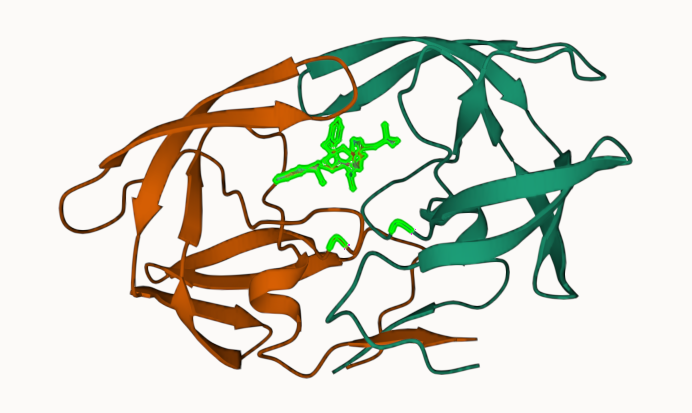
\includegraphics{1HSG.png}

}

\caption{HIV-Pr structure from 1hsg}

\end{figure}

\hypertarget{introduction-to-bio3d-in-r}{%
\subsection{3. Introduction to Bio3D in
R}\label{introduction-to-bio3d-in-r}}

Bio3D is an R package for structural bioinformatics. To use it we need
to call it with \texttt{library()} function (just like any package).

\begin{Shaded}
\begin{Highlighting}[]
\FunctionTok{library}\NormalTok{(}\StringTok{\textquotesingle{}bio3d\textquotesingle{}}\NormalTok{)}
\end{Highlighting}
\end{Shaded}

TO read a PDB file we can use \texttt{read.pdb()}

\begin{Shaded}
\begin{Highlighting}[]
\NormalTok{pdb }\OtherTok{\textless{}{-}} \FunctionTok{read.pdb}\NormalTok{(}\StringTok{\textquotesingle{}1hsg\textquotesingle{}}\NormalTok{)}
\end{Highlighting}
\end{Shaded}

\begin{verbatim}
  Note: Accessing on-line PDB file
\end{verbatim}

\begin{Shaded}
\begin{Highlighting}[]
\NormalTok{pdb}
\end{Highlighting}
\end{Shaded}

\begin{verbatim}

 Call:  read.pdb(file = "1hsg")

   Total Models#: 1
     Total Atoms#: 1686,  XYZs#: 5058  Chains#: 2  (values: A B)

     Protein Atoms#: 1514  (residues/Calpha atoms#: 198)
     Nucleic acid Atoms#: 0  (residues/phosphate atoms#: 0)

     Non-protein/nucleic Atoms#: 172  (residues: 128)
     Non-protein/nucleic resid values: [ HOH (127), MK1 (1) ]

   Protein sequence:
      PQITLWQRPLVTIKIGGQLKEALLDTGADDTVLEEMSLPGRWKPKMIGGIGGFIKVRQYD
      QILIEICGHKAIGTVLVGPTPVNIIGRNLLTQIGCTLNFPQITLWQRPLVTIKIGGQLKE
      ALLDTGADDTVLEEMSLPGRWKPKMIGGIGGFIKVRQYDQILIEICGHKAIGTVLVGPTP
      VNIIGRNLLTQIGCTLNF

+ attr: atom, xyz, seqres, helix, sheet,
        calpha, remark, call
\end{verbatim}

\begin{quote}
Q7: How many amino acid residues are there in this pdb object?
\end{quote}

There are 198 amino acids

\begin{quote}
Q8: Name one of the two non-protein residues?
\end{quote}

One of the two non-protein residues is MK1, the drug ligand.

\begin{quote}
Q9: How many protein chains are in this structure?
\end{quote}

Threre are two chains in this protein structure.

\begin{Shaded}
\begin{Highlighting}[]
\FunctionTok{attributes}\NormalTok{(pdb)}
\end{Highlighting}
\end{Shaded}

\begin{verbatim}
$names
[1] "atom"   "xyz"    "seqres" "helix"  "sheet"  "calpha" "remark" "call"  

$class
[1] "pdb" "sse"
\end{verbatim}

THe ATOM records of a PDB file are stored in \texttt{pdb\$atom}

\begin{Shaded}
\begin{Highlighting}[]
\FunctionTok{head}\NormalTok{(pdb}\SpecialCharTok{$}\NormalTok{atom)}
\end{Highlighting}
\end{Shaded}

\begin{verbatim}
  type eleno elety  alt resid chain resno insert      x      y     z o     b
1 ATOM     1     N <NA>   PRO     A     1   <NA> 29.361 39.686 5.862 1 38.10
2 ATOM     2    CA <NA>   PRO     A     1   <NA> 30.307 38.663 5.319 1 40.62
3 ATOM     3     C <NA>   PRO     A     1   <NA> 29.760 38.071 4.022 1 42.64
4 ATOM     4     O <NA>   PRO     A     1   <NA> 28.600 38.302 3.676 1 43.40
5 ATOM     5    CB <NA>   PRO     A     1   <NA> 30.508 37.541 6.342 1 37.87
6 ATOM     6    CG <NA>   PRO     A     1   <NA> 29.296 37.591 7.162 1 38.40
  segid elesy charge
1  <NA>     N   <NA>
2  <NA>     C   <NA>
3  <NA>     C   <NA>
4  <NA>     O   <NA>
5  <NA>     C   <NA>
6  <NA>     C   <NA>
\end{verbatim}

\hypertarget{comparative-structure-analysis-of-adenylate-kinase-adk}{%
\subsection{4. Comparative structure analysis of Adenylate Kinase
(ADK)}\label{comparative-structure-analysis-of-adenylate-kinase-adk}}

Installed packages in console.

\begin{quote}
Q10. Which of the packages above is found only on BioConductor and not
CRAN?
\end{quote}

msa is found only on BioConductor and not CRAN.

\begin{quote}
Q11. Which of the above packages is not found on BioConductor or CRAN?
\end{quote}

bio3d-view is not found on BioConductor or CRAN.

\begin{quote}
Q12. True or False? Functions from the devtools package can be used to
install packages from GitHub and BitBucket?
\end{quote}

TRUE.

We will start our analysis with a single PDB id (code from the PDB
database): 1AKE

First we get it's primary sequence:

\begin{Shaded}
\begin{Highlighting}[]
\NormalTok{aa }\OtherTok{\textless{}{-}} \FunctionTok{get.seq}\NormalTok{(}\StringTok{\textquotesingle{}1ake\_a\textquotesingle{}}\NormalTok{)}
\end{Highlighting}
\end{Shaded}

\begin{verbatim}
Warning in get.seq("1ake_a"): Removing existing file: seqs.fasta
\end{verbatim}

\begin{verbatim}
Fetching... Please wait. Done.
\end{verbatim}

\begin{Shaded}
\begin{Highlighting}[]
\NormalTok{aa}
\end{Highlighting}
\end{Shaded}

\begin{verbatim}
             1        .         .         .         .         .         60 
pdb|1AKE|A   MRIILLGAPGAGKGTQAQFIMEKYGIPQISTGDMLRAAVKSGSELGKQAKDIMDAGKLVT
             1        .         .         .         .         .         60 

            61        .         .         .         .         .         120 
pdb|1AKE|A   DELVIALVKERIAQEDCRNGFLLDGFPRTIPQADAMKEAGINVDYVLEFDVPDELIVDRI
            61        .         .         .         .         .         120 

           121        .         .         .         .         .         180 
pdb|1AKE|A   VGRRVHAPSGRVYHVKFNPPKVEGKDDVTGEELTTRKDDQEETVRKRLVEYHQMTAPLIG
           121        .         .         .         .         .         180 

           181        .         .         .   214 
pdb|1AKE|A   YYSKEAEAGNTKYAKVDGTKPVAEVRADLEKILG
           181        .         .         .   214 

Call:
  read.fasta(file = outfile)

Class:
  fasta

Alignment dimensions:
  1 sequence rows; 214 position columns (214 non-gap, 0 gap) 

+ attr: id, ali, call
\end{verbatim}

\begin{quote}
Q13. How many amino acids are in this sequence, i.e.~how long is this
sequence?
\end{quote}

There are 214 amino acids in this sequence.

\begin{Shaded}
\begin{Highlighting}[]
\CommentTok{\# Blast or hmmer search}
\NormalTok{b }\OtherTok{\textless{}{-}} \FunctionTok{blast.pdb}\NormalTok{(aa)}
\end{Highlighting}
\end{Shaded}

\begin{verbatim}
 Searching ... please wait (updates every 5 seconds) RID = NNM6A3A5016 
 .........
 Reporting 98 hits
\end{verbatim}

\begin{Shaded}
\begin{Highlighting}[]
\NormalTok{hits }\OtherTok{\textless{}{-}}  \FunctionTok{plot}\NormalTok{(b)}
\end{Highlighting}
\end{Shaded}

\begin{verbatim}
  * Possible cutoff values:    197 -3 
            Yielding Nhits:    16 98 

  * Chosen cutoff value of:    197 
            Yielding Nhits:    16 
\end{verbatim}

\begin{figure}[H]

{\centering 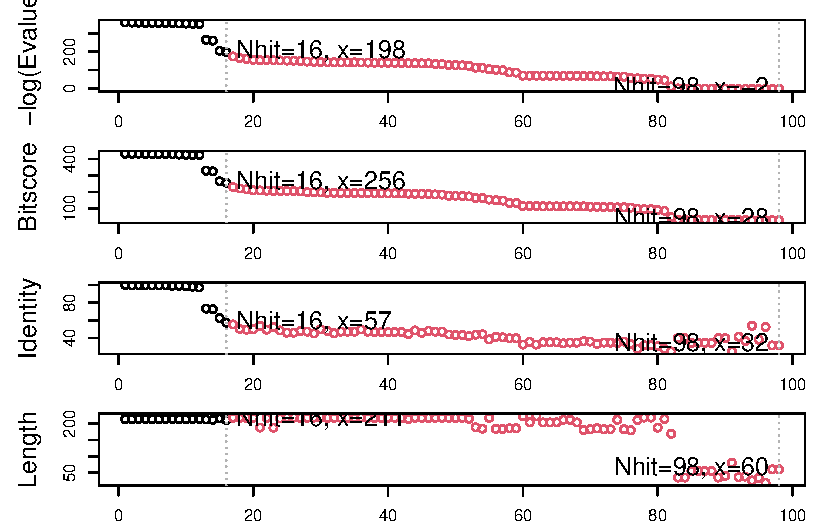
\includegraphics{class09_files/figure-pdf/unnamed-chunk-8-1.pdf}

}

\end{figure}

\begin{Shaded}
\begin{Highlighting}[]
\CommentTok{\# List out some \textquotesingle{}top hits\textquotesingle{}}
\CommentTok{\# head(hits$pdb.id)}
\end{Highlighting}
\end{Shaded}

Use these ADK structures for analysis

\begin{Shaded}
\begin{Highlighting}[]
\NormalTok{hits }\OtherTok{\textless{}{-}}  \ConstantTok{NULL}
\NormalTok{hits}\SpecialCharTok{$}\NormalTok{pdb.id }\OtherTok{\textless{}{-}}  \FunctionTok{c}\NormalTok{(}\StringTok{\textquotesingle{}1AKE\_A\textquotesingle{}}\NormalTok{,}\StringTok{\textquotesingle{}6S36\_A\textquotesingle{}}\NormalTok{,}\StringTok{\textquotesingle{}6RZE\_A\textquotesingle{}}\NormalTok{,}\StringTok{\textquotesingle{}3HPR\_A\textquotesingle{}}\NormalTok{,}\StringTok{\textquotesingle{}1E4V\_A\textquotesingle{}}\NormalTok{,}\StringTok{\textquotesingle{}5EJE\_A\textquotesingle{}}\NormalTok{,}\StringTok{\textquotesingle{}1E4Y\_A\textquotesingle{}}\NormalTok{,}\StringTok{\textquotesingle{}3X2S\_A\textquotesingle{}}\NormalTok{,}\StringTok{\textquotesingle{}6HAP\_A\textquotesingle{}}\NormalTok{,}\StringTok{\textquotesingle{}6HAM\_A\textquotesingle{}}\NormalTok{,}\StringTok{\textquotesingle{}4K46\_A\textquotesingle{}}\NormalTok{,}\StringTok{\textquotesingle{}3GMT\_A\textquotesingle{}}\NormalTok{,}\StringTok{\textquotesingle{}4PZL\_A\textquotesingle{}}\NormalTok{)}
\end{Highlighting}
\end{Shaded}

Download all these PDB files from the online database

\begin{Shaded}
\begin{Highlighting}[]
\CommentTok{\# Download related PDB files}
\NormalTok{files }\OtherTok{\textless{}{-}} \FunctionTok{get.pdb}\NormalTok{(hits}\SpecialCharTok{$}\NormalTok{pdb.id, }\AttributeTok{path=}\StringTok{\textquotesingle{}pdbs\textquotesingle{}}\NormalTok{, }\AttributeTok{split=}\ConstantTok{TRUE}\NormalTok{, }\AttributeTok{gzip=}\ConstantTok{TRUE}\NormalTok{)}
\end{Highlighting}
\end{Shaded}

\begin{verbatim}
Warning in get.pdb(hits$pdb.id, path = "pdbs", split = TRUE, gzip = TRUE): pdbs/
1AKE.pdb.gz exists. Skipping download
\end{verbatim}

\begin{verbatim}
Warning in get.pdb(hits$pdb.id, path = "pdbs", split = TRUE, gzip = TRUE): pdbs/
6S36.pdb.gz exists. Skipping download
\end{verbatim}

\begin{verbatim}
Warning in get.pdb(hits$pdb.id, path = "pdbs", split = TRUE, gzip = TRUE): pdbs/
6RZE.pdb.gz exists. Skipping download
\end{verbatim}

\begin{verbatim}
Warning in get.pdb(hits$pdb.id, path = "pdbs", split = TRUE, gzip = TRUE): pdbs/
3HPR.pdb.gz exists. Skipping download
\end{verbatim}

\begin{verbatim}
Warning in get.pdb(hits$pdb.id, path = "pdbs", split = TRUE, gzip = TRUE): pdbs/
1E4V.pdb.gz exists. Skipping download
\end{verbatim}

\begin{verbatim}
Warning in get.pdb(hits$pdb.id, path = "pdbs", split = TRUE, gzip = TRUE): pdbs/
5EJE.pdb.gz exists. Skipping download
\end{verbatim}

\begin{verbatim}
Warning in get.pdb(hits$pdb.id, path = "pdbs", split = TRUE, gzip = TRUE): pdbs/
1E4Y.pdb.gz exists. Skipping download
\end{verbatim}

\begin{verbatim}
Warning in get.pdb(hits$pdb.id, path = "pdbs", split = TRUE, gzip = TRUE): pdbs/
3X2S.pdb.gz exists. Skipping download
\end{verbatim}

\begin{verbatim}
Warning in get.pdb(hits$pdb.id, path = "pdbs", split = TRUE, gzip = TRUE): pdbs/
6HAP.pdb.gz exists. Skipping download
\end{verbatim}

\begin{verbatim}
Warning in get.pdb(hits$pdb.id, path = "pdbs", split = TRUE, gzip = TRUE): pdbs/
6HAM.pdb.gz exists. Skipping download
\end{verbatim}

\begin{verbatim}
Warning in get.pdb(hits$pdb.id, path = "pdbs", split = TRUE, gzip = TRUE): pdbs/
4K46.pdb.gz exists. Skipping download
\end{verbatim}

\begin{verbatim}
Warning in get.pdb(hits$pdb.id, path = "pdbs", split = TRUE, gzip = TRUE): pdbs/
3GMT.pdb.gz exists. Skipping download
\end{verbatim}

\begin{verbatim}
Warning in get.pdb(hits$pdb.id, path = "pdbs", split = TRUE, gzip = TRUE): pdbs/
4PZL.pdb.gz exists. Skipping download
\end{verbatim}

\begin{verbatim}

  |                                                                            
  |                                                                      |   0%
  |                                                                            
  |=====                                                                 |   8%
  |                                                                            
  |===========                                                           |  15%
  |                                                                            
  |================                                                      |  23%
  |                                                                            
  |======================                                                |  31%
  |                                                                            
  |===========================                                           |  38%
  |                                                                            
  |================================                                      |  46%
  |                                                                            
  |======================================                                |  54%
  |                                                                            
  |===========================================                           |  62%
  |                                                                            
  |================================================                      |  69%
  |                                                                            
  |======================================================                |  77%
  |                                                                            
  |===========================================================           |  85%
  |                                                                            
  |=================================================================     |  92%
  |                                                                            
  |======================================================================| 100%
\end{verbatim}

\hypertarget{align-and-superose-structures}{%
\subsubsection{Align and superose
structures}\label{align-and-superose-structures}}

Align all these structures

\begin{Shaded}
\begin{Highlighting}[]
\CommentTok{\# Align releated PDBs}
\NormalTok{pdbs }\OtherTok{\textless{}{-}} \FunctionTok{pdbaln}\NormalTok{(files, }\AttributeTok{fit =} \ConstantTok{TRUE}\NormalTok{, }\AttributeTok{exefile=}\StringTok{"msa"}\NormalTok{)}
\end{Highlighting}
\end{Shaded}

\begin{verbatim}
Reading PDB files:
pdbs/split_chain/1AKE_A.pdb
pdbs/split_chain/6S36_A.pdb
pdbs/split_chain/6RZE_A.pdb
pdbs/split_chain/3HPR_A.pdb
pdbs/split_chain/1E4V_A.pdb
pdbs/split_chain/5EJE_A.pdb
pdbs/split_chain/1E4Y_A.pdb
pdbs/split_chain/3X2S_A.pdb
pdbs/split_chain/6HAP_A.pdb
pdbs/split_chain/6HAM_A.pdb
pdbs/split_chain/4K46_A.pdb
pdbs/split_chain/3GMT_A.pdb
pdbs/split_chain/4PZL_A.pdb
   PDB has ALT records, taking A only, rm.alt=TRUE
.   PDB has ALT records, taking A only, rm.alt=TRUE
.   PDB has ALT records, taking A only, rm.alt=TRUE
.   PDB has ALT records, taking A only, rm.alt=TRUE
..   PDB has ALT records, taking A only, rm.alt=TRUE
....   PDB has ALT records, taking A only, rm.alt=TRUE
.   PDB has ALT records, taking A only, rm.alt=TRUE
...

Extracting sequences

pdb/seq: 1   name: pdbs/split_chain/1AKE_A.pdb 
   PDB has ALT records, taking A only, rm.alt=TRUE
pdb/seq: 2   name: pdbs/split_chain/6S36_A.pdb 
   PDB has ALT records, taking A only, rm.alt=TRUE
pdb/seq: 3   name: pdbs/split_chain/6RZE_A.pdb 
   PDB has ALT records, taking A only, rm.alt=TRUE
pdb/seq: 4   name: pdbs/split_chain/3HPR_A.pdb 
   PDB has ALT records, taking A only, rm.alt=TRUE
pdb/seq: 5   name: pdbs/split_chain/1E4V_A.pdb 
pdb/seq: 6   name: pdbs/split_chain/5EJE_A.pdb 
   PDB has ALT records, taking A only, rm.alt=TRUE
pdb/seq: 7   name: pdbs/split_chain/1E4Y_A.pdb 
pdb/seq: 8   name: pdbs/split_chain/3X2S_A.pdb 
pdb/seq: 9   name: pdbs/split_chain/6HAP_A.pdb 
pdb/seq: 10   name: pdbs/split_chain/6HAM_A.pdb 
   PDB has ALT records, taking A only, rm.alt=TRUE
pdb/seq: 11   name: pdbs/split_chain/4K46_A.pdb 
   PDB has ALT records, taking A only, rm.alt=TRUE
pdb/seq: 12   name: pdbs/split_chain/3GMT_A.pdb 
pdb/seq: 13   name: pdbs/split_chain/4PZL_A.pdb 
\end{verbatim}

\begin{Shaded}
\begin{Highlighting}[]
\CommentTok{\# Vector containing PDB codes for figure axis}
\NormalTok{ids }\OtherTok{\textless{}{-}} \FunctionTok{basename.pdb}\NormalTok{(pdbs}\SpecialCharTok{$}\NormalTok{id)}

\FunctionTok{dev.off}\NormalTok{()}
\end{Highlighting}
\end{Shaded}

\begin{verbatim}
null device 
          1 
\end{verbatim}

\begin{Shaded}
\begin{Highlighting}[]
\CommentTok{\# Draw schematic alignment}
\FunctionTok{plot}\NormalTok{(pdbs, }\AttributeTok{labels=}\NormalTok{ids)}

\CommentTok{\# adjust plot margins}
\FunctionTok{par}\NormalTok{(}\AttributeTok{mar =} \FunctionTok{c}\NormalTok{(}\DecValTok{1}\NormalTok{,}\DecValTok{1}\NormalTok{,}\DecValTok{1}\NormalTok{,}\DecValTok{1}\NormalTok{))}
\end{Highlighting}
\end{Shaded}

\hypertarget{annotate-collected-pdb-structures}{%
\subsubsection{Annotate collected PDB
structures}\label{annotate-collected-pdb-structures}}

Annotating structures

\begin{Shaded}
\begin{Highlighting}[]
\NormalTok{anno }\OtherTok{\textless{}{-}} \FunctionTok{pdb.annotate}\NormalTok{(ids)}
\FunctionTok{unique}\NormalTok{(anno}\SpecialCharTok{$}\NormalTok{source)}
\end{Highlighting}
\end{Shaded}

\begin{verbatim}
[1] "Escherichia coli"                                
[2] "Escherichia coli K-12"                           
[3] "Escherichia coli O139:H28 str. E24377A"          
[4] "Escherichia coli str. K-12 substr. MDS42"        
[5] "Photobacterium profundum"                        
[6] "Burkholderia pseudomallei 1710b"                 
[7] "Francisella tularensis subsp. tularensis SCHU S4"
\end{verbatim}

Viewing all available annotation data:

\begin{Shaded}
\begin{Highlighting}[]
\NormalTok{anno}
\end{Highlighting}
\end{Shaded}

\begin{verbatim}
       structureId chainId macromoleculeType chainLength experimentalTechnique
1AKE_A        1AKE       A           Protein         214                 X-ray
6S36_A        6S36       A           Protein         214                 X-ray
6RZE_A        6RZE       A           Protein         214                 X-ray
3HPR_A        3HPR       A           Protein         214                 X-ray
1E4V_A        1E4V       A           Protein         214                 X-ray
5EJE_A        5EJE       A           Protein         214                 X-ray
1E4Y_A        1E4Y       A           Protein         214                 X-ray
3X2S_A        3X2S       A           Protein         214                 X-ray
6HAP_A        6HAP       A           Protein         214                 X-ray
6HAM_A        6HAM       A           Protein         214                 X-ray
4K46_A        4K46       A           Protein         214                 X-ray
3GMT_A        3GMT       A           Protein         230                 X-ray
4PZL_A        4PZL       A           Protein         242                 X-ray
       resolution       scopDomain                                        pfam
1AKE_A       2.00 Adenylate kinase Adenylate kinase, active site lid (ADK_lid)
6S36_A       1.60             <NA> Adenylate kinase, active site lid (ADK_lid)
6RZE_A       1.69             <NA> Adenylate kinase, active site lid (ADK_lid)
3HPR_A       2.00             <NA> Adenylate kinase, active site lid (ADK_lid)
1E4V_A       1.85 Adenylate kinase Adenylate kinase, active site lid (ADK_lid)
5EJE_A       1.90             <NA> Adenylate kinase, active site lid (ADK_lid)
1E4Y_A       1.85 Adenylate kinase Adenylate kinase, active site lid (ADK_lid)
3X2S_A       2.80             <NA> Adenylate kinase, active site lid (ADK_lid)
6HAP_A       2.70             <NA> Adenylate kinase, active site lid (ADK_lid)
6HAM_A       2.55             <NA> Adenylate kinase, active site lid (ADK_lid)
4K46_A       2.01             <NA> Adenylate kinase, active site lid (ADK_lid)
3GMT_A       2.10             <NA> Adenylate kinase, active site lid (ADK_lid)
4PZL_A       2.10             <NA> Adenylate kinase, active site lid (ADK_lid)
               ligandId
1AKE_A              AP5
6S36_A CL (3),NA,MG (2)
6RZE_A    NA (3),CL (2)
3HPR_A              AP5
1E4V_A              AP5
5EJE_A           AP5,CO
1E4Y_A              AP5
3X2S_A   JPY (2),AP5,MG
6HAP_A              AP5
6HAM_A              AP5
4K46_A      ADP,AMP,PO4
3GMT_A          SO4 (2)
4PZL_A       CA,FMT,GOL
                                                                             ligandName
1AKE_A                                                 BIS(ADENOSINE)-5'-PENTAPHOSPHATE
6S36_A                                    CHLORIDE ION (3),SODIUM ION,MAGNESIUM ION (2)
6RZE_A                                                  SODIUM ION (3),CHLORIDE ION (2)
3HPR_A                                                 BIS(ADENOSINE)-5'-PENTAPHOSPHATE
1E4V_A                                                 BIS(ADENOSINE)-5'-PENTAPHOSPHATE
5EJE_A                                 BIS(ADENOSINE)-5'-PENTAPHOSPHATE,COBALT (II) ION
1E4Y_A                                                 BIS(ADENOSINE)-5'-PENTAPHOSPHATE
3X2S_A N-(pyren-1-ylmethyl)acetamide (2),BIS(ADENOSINE)-5'-PENTAPHOSPHATE,MAGNESIUM ION
6HAP_A                                                 BIS(ADENOSINE)-5'-PENTAPHOSPHATE
6HAM_A                                                 BIS(ADENOSINE)-5'-PENTAPHOSPHATE
4K46_A                   ADENOSINE-5'-DIPHOSPHATE,ADENOSINE MONOPHOSPHATE,PHOSPHATE ION
3GMT_A                                                                  SULFATE ION (2)
4PZL_A                                                 CALCIUM ION,FORMIC ACID,GLYCEROL
                                                 source
1AKE_A                                 Escherichia coli
6S36_A                                 Escherichia coli
6RZE_A                                 Escherichia coli
3HPR_A                            Escherichia coli K-12
1E4V_A                                 Escherichia coli
5EJE_A           Escherichia coli O139:H28 str. E24377A
1E4Y_A                                 Escherichia coli
3X2S_A         Escherichia coli str. K-12 substr. MDS42
6HAP_A           Escherichia coli O139:H28 str. E24377A
6HAM_A                            Escherichia coli K-12
4K46_A                         Photobacterium profundum
3GMT_A                  Burkholderia pseudomallei 1710b
4PZL_A Francisella tularensis subsp. tularensis SCHU S4
                                                                                                                                                                     structureTitle
1AKE_A STRUCTURE OF THE COMPLEX BETWEEN ADENYLATE KINASE FROM ESCHERICHIA COLI AND THE INHIBITOR AP5A REFINED AT 1.9 ANGSTROMS RESOLUTION: A MODEL FOR A CATALYTIC TRANSITION STATE
6S36_A                                                                                                                   Crystal structure of E. coli Adenylate kinase R119K mutant
6RZE_A                                                                                                                   Crystal structure of E. coli Adenylate kinase R119A mutant
3HPR_A                                                                                               Crystal structure of V148G adenylate kinase from E. coli, in complex with Ap5A
1E4V_A                                                                                                       Mutant G10V of adenylate kinase from E. coli, modified in the Gly-loop
5EJE_A                                                                                  Crystal structure of E. coli Adenylate kinase G56C/T163C double mutant in complex with Ap5a
1E4Y_A                                                                                                        Mutant P9L of adenylate kinase from E. coli, modified in the Gly-loop
3X2S_A                                                                                                                      Crystal structure of pyrene-conjugated adenylate kinase
6HAP_A                                                                                                                                                             Adenylate kinase
6HAM_A                                                                                                                                                             Adenylate kinase
4K46_A                                                                                                          Crystal Structure of Adenylate Kinase from Photobacterium profundum
3GMT_A                                                                                                         Crystal structure of adenylate kinase from burkholderia pseudomallei
4PZL_A                                                                              The crystal structure of adenylate kinase from Francisella tularensis subsp. tularensis SCHU S4
                                                     citation rObserved   rFree
1AKE_A                 Muller, C.W., et al. J Mol Biol (1992)   0.19600      NA
6S36_A                  Rogne, P., et al. Biochemistry (2019)   0.16320 0.23560
6RZE_A                  Rogne, P., et al. Biochemistry (2019)   0.18650 0.23500
3HPR_A  Schrank, T.P., et al. Proc Natl Acad Sci U S A (2009)   0.21000 0.24320
1E4V_A                   Muller, C.W., et al. Proteins (1993)   0.19600      NA
5EJE_A  Kovermann, M., et al. Proc Natl Acad Sci U S A (2017)   0.18890 0.23580
1E4Y_A                   Muller, C.W., et al. Proteins (1993)   0.17800      NA
3X2S_A                Fujii, A., et al. Bioconjug Chem (2015)   0.20700 0.25600
6HAP_A               Kantaev, R., et al. J Phys Chem B (2018)   0.22630 0.27760
6HAM_A               Kantaev, R., et al. J Phys Chem B (2018)   0.20511 0.24325
4K46_A                    Cho, Y.-J., et al. To be published    0.17000 0.22290
3GMT_A Buchko, G.W., et al. Biochem Biophys Res Commun (2010)   0.23800 0.29500
4PZL_A                       Tan, K., et al. To be published    0.19360 0.23680
         rWork spaceGroup
1AKE_A 0.19600  P 21 2 21
6S36_A 0.15940    C 1 2 1
6RZE_A 0.18190    C 1 2 1
3HPR_A 0.20620  P 21 21 2
1E4V_A 0.19600  P 21 2 21
5EJE_A 0.18630  P 21 2 21
1E4Y_A 0.17800   P 1 21 1
3X2S_A 0.20700 P 21 21 21
6HAP_A 0.22370    I 2 2 2
6HAM_A 0.20311       P 43
4K46_A 0.16730 P 21 21 21
3GMT_A 0.23500   P 1 21 1
4PZL_A 0.19130       P 32
\end{verbatim}

\hypertarget{principal-component-analysis}{%
\subsubsection{Principal Component
analysis}\label{principal-component-analysis}}

Performing PCA

\begin{Shaded}
\begin{Highlighting}[]
\CommentTok{\# Perform PCA}
\NormalTok{pc.xray }\OtherTok{\textless{}{-}} \FunctionTok{pca}\NormalTok{(pdbs)}
\FunctionTok{plot}\NormalTok{(pc.xray)}
\end{Highlighting}
\end{Shaded}

\begin{figure}[H]

{\centering 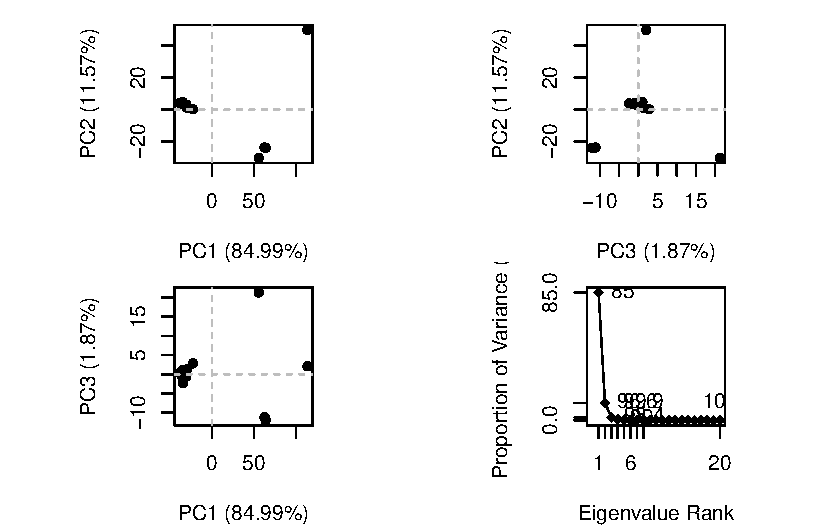
\includegraphics{class09_files/figure-pdf/unnamed-chunk-15-1.pdf}

}

\end{figure}

Calculating pairwise RMSD values

\begin{Shaded}
\begin{Highlighting}[]
\CommentTok{\# Calculate RMSD}
\NormalTok{rd }\OtherTok{\textless{}{-}} \FunctionTok{rmsd}\NormalTok{(pdbs)}
\end{Highlighting}
\end{Shaded}

\begin{verbatim}
Warning in rmsd(pdbs): No indices provided, using the 204 non NA positions
\end{verbatim}

\begin{Shaded}
\begin{Highlighting}[]
\CommentTok{\# Structure{-}based clustering}
\NormalTok{hc.rd }\OtherTok{\textless{}{-}} \FunctionTok{hclust}\NormalTok{(}\FunctionTok{dist}\NormalTok{(rd))}
\NormalTok{grps.rd }\OtherTok{\textless{}{-}} \FunctionTok{cutree}\NormalTok{(hc.rd, }\AttributeTok{k=}\DecValTok{3}\NormalTok{)}

\FunctionTok{plot}\NormalTok{(pc.xray, }\DecValTok{1}\SpecialCharTok{:}\DecValTok{2}\NormalTok{, }\AttributeTok{col=}\StringTok{"grey50"}\NormalTok{, }\AttributeTok{bg=}\NormalTok{grps.rd, }\AttributeTok{pch=}\DecValTok{21}\NormalTok{, }\AttributeTok{cex=}\DecValTok{1}\NormalTok{)}
\end{Highlighting}
\end{Shaded}

\begin{figure}[H]

{\centering 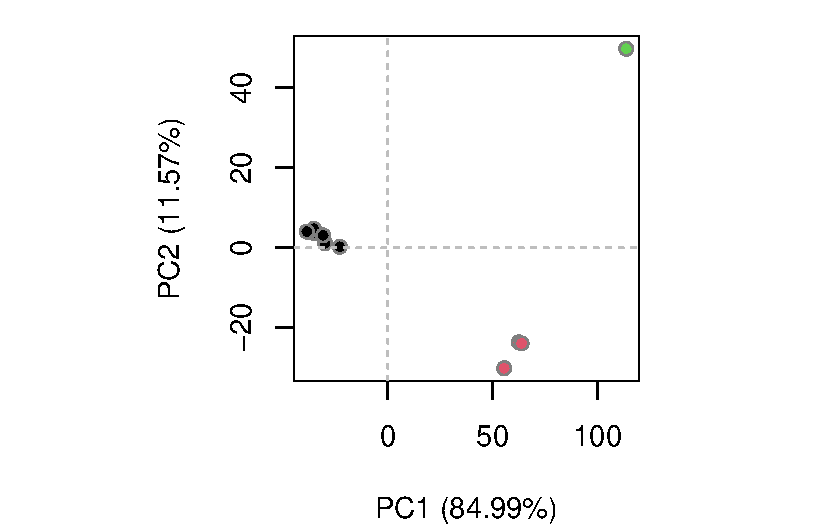
\includegraphics{class09_files/figure-pdf/unnamed-chunk-16-1.pdf}

}

\end{figure}

\hypertarget{optional-further-visualization}{%
\subsection{5. Optional Further
Visualization}\label{optional-further-visualization}}

Trying to visualize major structural variation

\begin{Shaded}
\begin{Highlighting}[]
\CommentTok{\# Visualize first principal component}
\NormalTok{pc1 }\OtherTok{\textless{}{-}} \FunctionTok{mktrj}\NormalTok{(pc.xray, }\AttributeTok{pc=}\DecValTok{1}\NormalTok{, }\AttributeTok{file=}\StringTok{"pc\_1.pdb"}\NormalTok{)}
\end{Highlighting}
\end{Shaded}

Animated visualizations

\begin{figure}

{\centering \includegraphics{PC_1.PDB_animate-trajectory.mp4}

}

\caption{Animated PC Visualization}

\end{figure}

Plotting main results with ggplot

\begin{Shaded}
\begin{Highlighting}[]
\CommentTok{\#Plotting results with ggplot2}
\FunctionTok{library}\NormalTok{(ggplot2)}
\FunctionTok{library}\NormalTok{(ggrepel)}

\NormalTok{df }\OtherTok{\textless{}{-}} \FunctionTok{data.frame}\NormalTok{(}\AttributeTok{PC1=}\NormalTok{pc.xray}\SpecialCharTok{$}\NormalTok{z[,}\DecValTok{1}\NormalTok{], }
                 \AttributeTok{PC2=}\NormalTok{pc.xray}\SpecialCharTok{$}\NormalTok{z[,}\DecValTok{2}\NormalTok{], }
                 \AttributeTok{col=}\FunctionTok{as.factor}\NormalTok{(grps.rd),}
                 \AttributeTok{ids=}\NormalTok{ids)}

\NormalTok{p }\OtherTok{\textless{}{-}} \FunctionTok{ggplot}\NormalTok{(df) }\SpecialCharTok{+} 
  \FunctionTok{aes}\NormalTok{(PC1, PC2, }\AttributeTok{col=}\NormalTok{col, }\AttributeTok{label=}\NormalTok{ids) }\SpecialCharTok{+}
  \FunctionTok{geom\_point}\NormalTok{(}\AttributeTok{size=}\DecValTok{2}\NormalTok{) }\SpecialCharTok{+}
  \FunctionTok{geom\_text\_repel}\NormalTok{(}\AttributeTok{max.overlaps =} \DecValTok{20}\NormalTok{) }\SpecialCharTok{+}
  \FunctionTok{theme}\NormalTok{(}\AttributeTok{legend.position =} \StringTok{"none"}\NormalTok{)}
\NormalTok{p}
\end{Highlighting}
\end{Shaded}

\begin{figure}[H]

{\centering 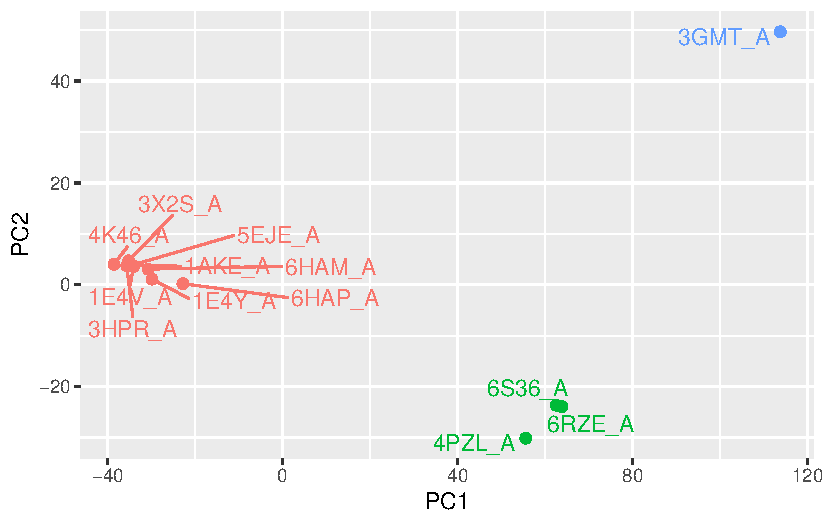
\includegraphics{class09_files/figure-pdf/unnamed-chunk-18-1.pdf}

}

\end{figure}

\hypertarget{normal-mode-analysis-optional}{%
\subsection{6. Normal mode analysis
{[}optional{]}}\label{normal-mode-analysis-optional}}

Doing NMA on pdbs

\begin{Shaded}
\begin{Highlighting}[]
\CommentTok{\# NMA of all structures}
\NormalTok{modes }\OtherTok{\textless{}{-}} \FunctionTok{nma}\NormalTok{(pdbs)}
\end{Highlighting}
\end{Shaded}

\begin{verbatim}

Details of Scheduled Calculation:
  ... 13 input structures 
  ... storing 606 eigenvectors for each structure 
  ... dimension of x$U.subspace: ( 612x606x13 )
  ... coordinate superposition prior to NM calculation 
  ... aligned eigenvectors (gap containing positions removed)  
  ... estimated memory usage of final 'eNMA' object: 36.9 Mb 


  |                                                                            
  |                                                                      |   0%
  |                                                                            
  |=====                                                                 |   8%
  |                                                                            
  |===========                                                           |  15%
  |                                                                            
  |================                                                      |  23%
  |                                                                            
  |======================                                                |  31%
  |                                                                            
  |===========================                                           |  38%
  |                                                                            
  |================================                                      |  46%
  |                                                                            
  |======================================                                |  54%
  |                                                                            
  |===========================================                           |  62%
  |                                                                            
  |================================================                      |  69%
  |                                                                            
  |======================================================                |  77%
  |                                                                            
  |===========================================================           |  85%
  |                                                                            
  |=================================================================     |  92%
  |                                                                            
  |======================================================================| 100%
\end{verbatim}

Plotting results

\begin{Shaded}
\begin{Highlighting}[]
\FunctionTok{plot}\NormalTok{(modes, pdbs, }\AttributeTok{col=}\NormalTok{grps.rd)}
\end{Highlighting}
\end{Shaded}

\begin{verbatim}
Extracting SSE from pdbs$sse attribute
\end{verbatim}

\begin{figure}[H]

{\centering 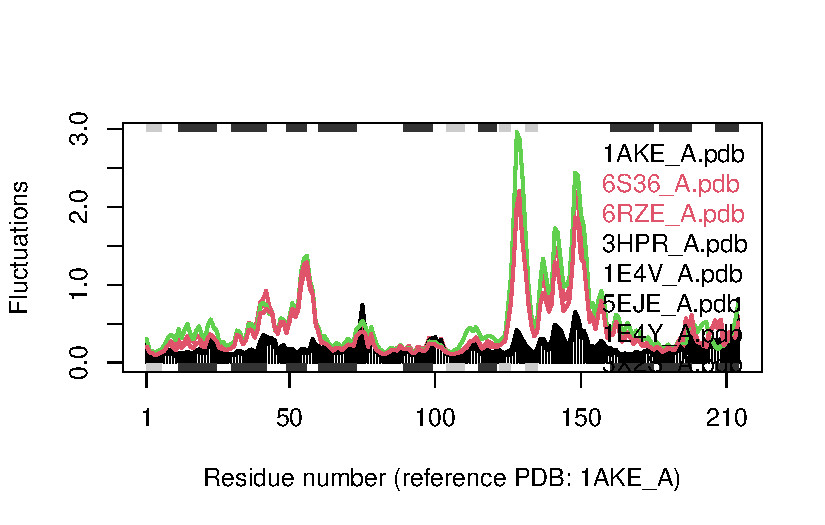
\includegraphics{class09_files/figure-pdf/unnamed-chunk-20-1.pdf}

}

\end{figure}

\begin{quote}
Q14. What do you note about this plot? Are the black and colored lines
similar or different? Where do you think they differ most and why?
\end{quote}

The black and colored lines are quite different. They seem to differ
most around residue number 40-50 and from 130-150. This is probably
because these are regions that change with the two major conformational
states for Adk. That is, they are the flexible binding-site regions that
would change their structure upon binding of a ligand. Therefore, those
regions exhibit a lot of fluctuation.



\end{document}
